% Compile on "nestor" which has the latest LaTeX distribution.
%    pdflatex brainbrowser-hbm2011poster.tex
%
\documentclass[a4shrink]{baposter}
%\documentclass[showframe]{baposter}
%\documentclass{baposter}

% \usepackage[vlined]{algorithm2e}
\usepackage{times}
\usepackage{calc}
\usepackage{url}
\usepackage{graphicx}
\usepackage{relsize}
\usepackage{multirow}
\usepackage{booktabs}
\usepackage{wrapfig}
\usepackage{floatflt}

\usepackage{graphicx}
\usepackage{multicol}
\usepackage[T1]{fontenc}
\usepackage{ae}

%\usepackage{helvet}
%\usepackage{bookman}
%\usepackage{palatino}

\graphicspath{{images/}}

%%%%%%%%%%%%%%%%%%%%%%%%%%%%%%%%%%%%%%%%%%%%%%%%%%%%%%%%%%%%%%%%%%%%%%%%%%%%%%%%
% Multicol Settings
%%%%%%%%%%%%%%%%%%%%%%%%%%%%%%%%%%%%%%%%%%%%%%%%%%%%%%%%%%%%%%%%%%%%%%%%%%%%%%%%
\setlength{\columnsep}{0.7em}
\setlength{\columnseprule}{0mm}

%%%%%%%%%%%%%%%%%%%%%%%%%%%%%%%%%%%%%%%%%%%%%%%%%%%%%%%%%%%%%%%%%%%%%%%%%%%%%%%%
% Save space in lists. Use this after the opening of the list
%%%%%%%%%%%%%%%%%%%%%%%%%%%%%%%%%%%%%%%%%%%%%%%%%%%%%%%%%%%%%%%%%%%%%%%%%%%%%%%%
\newcommand{\compresslist}{%
\setlength{\itemsep}{1pt}%
\setlength{\parskip}{0pt}%
\setlength{\parsep}{0pt}%
}

\newcommand{\Frac}[2]{\displaystyle{\frac{\displaystyle{#1}}
                                         {\displaystyle{#2}}}}
\newcommand{\Sum}[2]{\displaystyle{\sum_{#1}^{#2}}}

%%%%%%%%%%%%%%%%%%%%%%%%%%%%%%%%%%%%%%%%%%%%%%%%%%%%%%%%%%%%%%%%%%%%%%%%%%%%%%
%%% Begin of Document
%%%%%%%%%%%%%%%%%%%%%%%%%%%%%%%%%%%%%%%%%%%%%%%%%%%%%%%%%%%%%%%%%%%%%%%%%%%%%%

\begin{document}

\begin{poster}{
  grid=no,            % Show grid to help with alignment
  colspacing=1em,     % Column spacing
  headerColorOne=cyan!20!white!90!black,    % Color style
  borderColor=cyan!30!white!90!black,
  textborder=faded,                         % Format of textbox
  headerborder=open,                        % Format of text header
  headershape=roundedright,
  background=none,
  bgColorOne=cyan!10!white,
  headerheight=0.20\textheight,
  background=none,
  headershade=plain}%
%
% Eye Catcher
{}
%
% Title
{\sf\Huge BrainBrowser\\
    \huge Web-Based 3D Visualization for the MACACC Dataset and Other Surface Data \\
    \vspace{0.25em}
    \large {\tt{http://brainbrowser.cbrain.mcgill.ca/}}
    \vspace{0.25em}}
%
%
%
% Authors
{\sf\normalsize Nicolas Kassis, Gaolang Gong, Marc-Etienne Rousseau, Reza~Adalat and Alan~Evans\\
\small Montreal Neurological Institute, McGill University, Montr\'{e}al, 
       Qu\'{e}bec, Canada \\
    \vspace{0.25em}
  %%{\includegraphics[width=0.32\linewidth]{cbrain_logos.png}}
    \vspace{-3em}
}
%
% logos empty on right margin
{}

% Width of left inset image
% \setlength{\leftimgwidth}{0.78em+8.0em}

%%%%%%%%%%%%%%%%%%%%%%%%%%%%%%%%%%%%%%%%%%%%%%%%%%%%%%%%%%%%%%%%%%%%%%%%%%%%%%
%%% Now define the boxes that make up the poster
%%%---------------------------------------------------------------------------
%%% Each box has a name and can be placed absolutely or relatively.
%%% The only inconvenience is that you can only specify a relative position 
%%% towards an already declared box. So if you have a box attached to the 
%%% bottom, one to the top and a third one which should be in between, you 
%%% have to specify the top and bottom boxes before you specify the middle 
%%% box.
%%%%%%%%%%%%%%%%%%%%%%%%%%%%%%%%%%%%%%%%%%%%%%%%%%%%%%%%%%%%%%%%%%%%%%%%%%%%%%

%%%%%%%%%%%%%%%%%%%%%%%%%%%%%%%%%%%%%%%%%%%%%%%%%%%%%%%%%%%%%%%%%%%%%%%%%%%%%%
\headerbox{Introduction}{name=introduction,column=0,span=1.5,row=0}{
MACACC (mapping anatomical correlation across cerebral cortex) was previously proposed to characterize vertex-wise correlations of any cortical morphological descriptor (cortical thickness, area and volume) across subjects1. The correlations represent structural associations between a seed vertex and all other vertices.  We have now created a database of correlation maps for all surface vertices. To allow web access to this precalculated MACACC database, we have utilized new web technologies (WebGL3 and HTML5) to create a highly interactive real-time 3D interface for exploration of this database. Moreover, BrainBrowser (http://brainbrowser.cbrain.mcgill.ca) allows users to explore any data, functional or structural, expressed in MNI space.\vspace{0.3em}

\begin{center}
  \begin{tabular}{cc}
    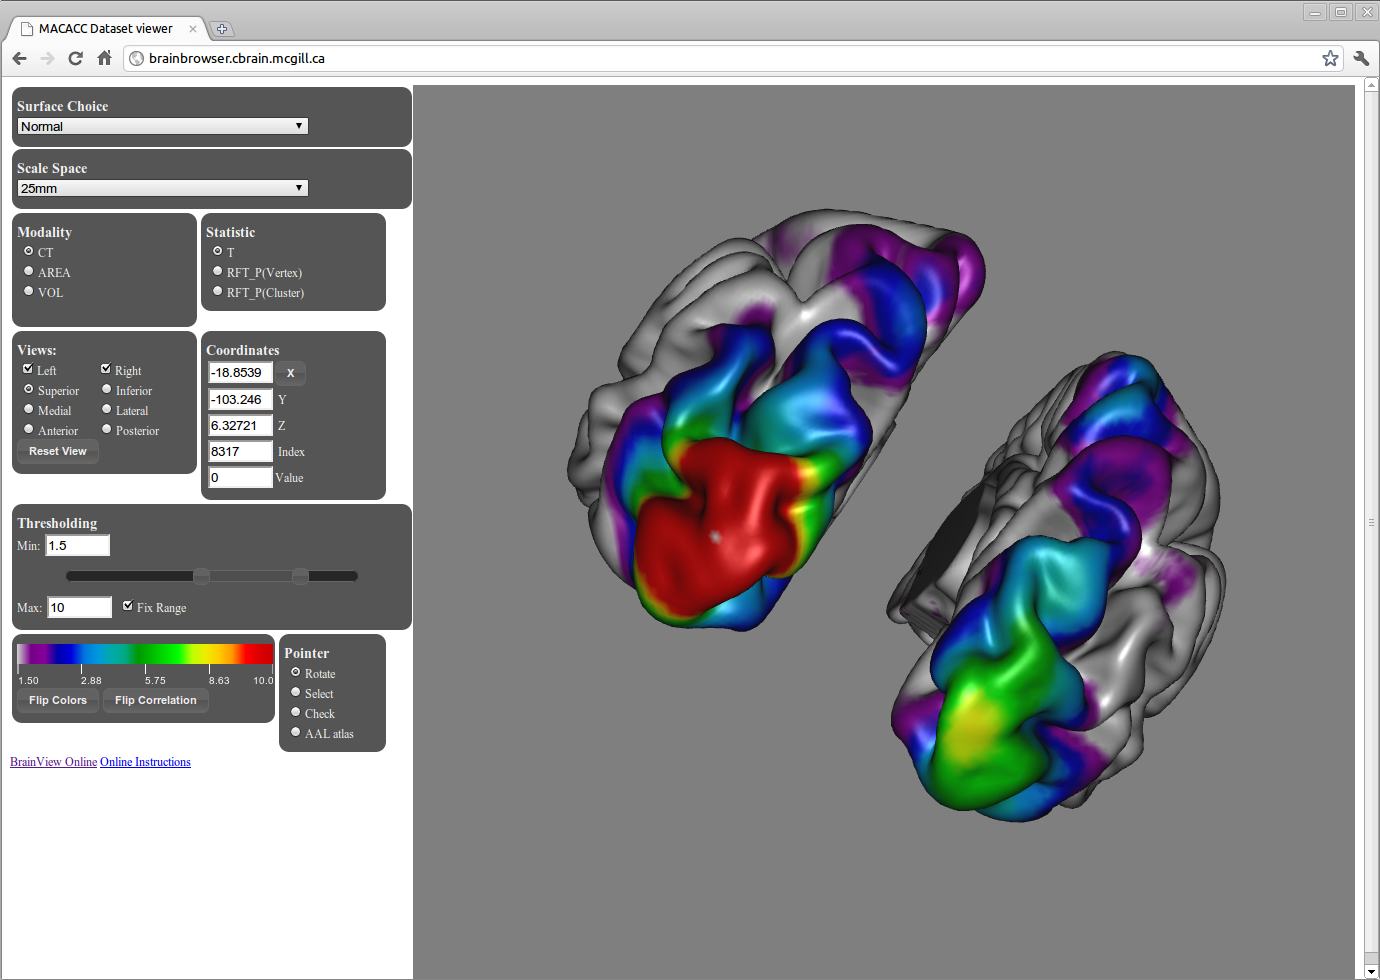
\includegraphics[width=1.0\linewidth]{macacc.png}
  \end{tabular}
\end{center}

}

%%%%%%%%%%%%%%%%%%%%%%%%%%%%%%%%%%%%%%%%%%%%%%%%%%%%%%%%%%%%%%%%%%%%%%%%%%%%%%

\headerbox{Methods}{name=management,column=1.5,span=1.5,row=0}{
The ICBM152 MRI dataset was used for the calculation of MACACC database. So far, we have included three vertex-wise morphological descriptors: cortical thickness, area and volume. For each descriptor, we calculated its vertex-wise Pearson correlation (in total 81924 vertices and therefore 81924 ⤬ 81924 correlations) after removing age, gender and global variables across the 152 subjects, using SurfStat2. We repeated the procedure for a range of smoothing kernels (FWHM = 0-40mm at 5mm intervals). 

BrainBrowser uses cutting-edge technologies such as WebGL and HTML5 which allow for the rendering and manipulation of 3D models within a web browser. These technologies are built into the latest versions of several popular browsers such as Chrome 9 and Firefox 4. Any user with access to the Internet will be able to visualize their data without any requirements for complex software installation or configuration locally.


\begin{center}
  \begin{tabular}{cc}
    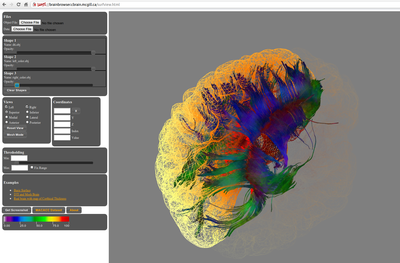
\includegraphics[width=1.0\linewidth]{brainbrowser.png}
  \end{tabular}
\end{center}
}

%%%%%%%%%%%%%%%%%%%%%%%%%%%%%%%%%%%%%%%%%%%%%%%%%%%%%%%%%%%%%%%%%%%%%%%%%%%%%%
\headerbox{Results}{name=collaboration,column=1.5,span=1.5,below=management}{
For each descriptor, the statistical maps of MACACC include t-statistic, p-value with and without random field theory correction. The data is formatted as text files that were stored on a file server at the MNI. BrainBrowser is now available online for anyone who requests remote access to the MACACC data, which is fast and highly interactive. Specifically, users can select any seeding vertex of a MACACC map on the cortical surface and further specify statistical thresholds (fig 1). Users can also use BrainBrowser to view surface data from their local machine (fig 2).

}


\end{poster}%
\end{document}
